\documentclass[11pt, english]{article}

\usepackage{multicol}
\usepackage{hyperref}
\usepackage[eng]{felipito}
\usepackage{stfloats}
\usepackage{mathpazo}

\usepackage[margin=0.8in, left=0.7in, right=0.7in]{geometry}

\graphicspath{{./Graphics/}}

% Colors
\definecolor{urlcolor}{rgb}{0,.145,.698}
\definecolor{linkcolor}{rgb}{.71,0.21,0.01}
\definecolor{citecolor}{rgb}{.12,.54,.11}


% Document title
\title{\bf Problem Set 1 \\ Statistics, Computation and
Applications\\[-1ex]}
\author{Felipe del Canto}
\date{September, 2021}
    
\hypersetup{
	breaklinks=true,  % so long urls are correctly broken across lines
    colorlinks=true,
    urlcolor=urlcolor,
    linkcolor=linkcolor,
    citecolor=citecolor,
}

\begin{document}
    
    \maketitle
    
    \hypertarget{problem-1.1-the-salk-vaccine-field-trial}{%
\section*{\texorpdfstring{\textbf{Problem 1.1:} The Salk Vaccine Field
Trial}{Problem 1.1: The Salk Vaccine Field Trial}}\label{problem-1.1-the-salk-vaccine-field-trial}}

The first polio epidemic hit the United States in 1916. By the 1950s
several vaccines against the disease had been discovered. The one
developed by Jonas Salk seemed the most promising in laboratory trials.
By 1954, the National Foundation for Infantile Paralysis (NFIP) was
ready to try the vaccine in the real world. They ran a controlled
experiment to analyze the effectiveness of the vaccine. The data is
shown in the table below (grade refers to the educational stage):

\begin{table}[H]
\caption{Table 1: NFIP study results.}
\centering
\begin{tabular}{lcc}
\toprule
& Size & Polio rate per 100,000 \\
\midrule
Grade 2 (vaccine) & 225,000 & 25 \\
Grades 1 and 3 (no vaccine) & 725,000 & 54 \\
Grade 2 (no consent) & 125,000 & 44 \\
\bottomrule
\end{tabular}
\end{table}

The experiment was later repeated as a randomized controlled
double-blind experiment. This data is shown in the second table below:

\begin{table}[H]
\caption{Table 2: Follow-up study results.}
\centering
\begin{tabular}{lcc}
\toprule
& Size & Polio rate per 100,000 \\
\midrule
Treatment (vaccine) & 200,000 & 28 \\
Control (salt injection) & 200,000 & 71 \\
No consent & 350,000 & 46 \\
\bottomrule
\end{tabular}
\end{table}

    \hypertarget{a-describe-each-of-the-two-studies-e.g.-their-design-and-comment-on-the-differences-between-them.-for-each-study-explain-whether-it-helps-measure-what-was-intended-to-be-estimated.}{%
\subparagraph{(a) Describe each of the two studies (e.g., their design)
and comment on the differences between them. For each study, explain
whether it helps measure what was intended to be
estimated.\\[2ex]}\label{a-describe-each-of-the-two-studies-e.g.-their-design-and-comment-on-the-differences-between-them.-for-each-study-explain-whether-it-helps-measure-what-was-intended-to-be-estimated.}}

    The NFIP study was not randomized: all students in grades 1 and 3 did
not get the vaccine, while the 2nd graders did. In that sense, the study
was not blinded, as both treatment and control groups knew their
assignment prior to treatment. Using this design, it is impossible to
detect to a greater level of confidence the effects of the vaccine. At
least two sources of bias can be identified for this design:
\begin{enumerate}
\item Students in 2nd grade are no necessarily comparable to younger or older
students, even from the same school. Differences can be related to
exposure to the virus but also to other confounders like gender
distribution, parents age and education, among other. This could imply
these students have different chances of getting polio, regardless the
vaccine, which will bias the results. In fact, comparing groups from
grades 1 and 3, with those from the no consent group, can lead us to
conclude these groups are not similar.

\item Being polio an infectious disease, peer effects can be substantial in
confounding the effects of the vaccine. This implies that students from
second grade that did not consent to the vaccine got protected by their
schoolmates by a weaker version of herd immunity. This could also affect
the rates of polio of 1st and 3rd graders if these students are
continuously sharing spaces at school. This could also be important if
students from the control and treatment groups both belong to the same
school.
\end{enumerate}
On the contrary, the follow-up experiment was double-blinded and
randomized. In this case, each student was randomly assigned to a
treatment group (and got the vaccine) or a control group (and got a
placebo). Observational data was obtained from those students that did
not consent to participate (the No consent group). A design like this
one is better suited to estimate the effects of the vaccine, as
potential confounders are now (in average) equal between both groups.
However, the second source of bias is not completely eliminated if
treatment is not randomized at school level. That is, if within the same
school there are children that belong to both treatment and control
groups, then the vaccine effect is biased downwards (i.e.~a lower bound
of its efficacy is estimated) due to peer effects. In that case,
vaccinated children indirectly protect those that only receive a salt
injection.

    \hypertarget{b-which-numbers-show-the-effectiveness-of-the-vaccine-explain-why.}{%
\subparagraph{(b) Which numbers show the effectiveness of the vaccine?
Explain
why. \\[2ex]}\label{b-which-numbers-show-the-effectiveness-of-the-vaccine-explain-why.}}

    The numbers capable of showing the effectiveness of the vaccine are
those in Table 2. However, which of these actually allow to test the
hypothesis depends on how the experiment was designed. If the
randomization occurred after asking for consent to participate, then we
would like to compare the rates of polio between treatment and control
groups. The caveat is that the sample that consented participating in
the study may have selected on particular characteristics, that could
bias the results in two possible ways:
\begin{enumerate}
\item If those that consented are people that could potentially benefit more
from the vaccine (e.g.~a family with previous close cases of polio) then
the effect would be larger (biased upwards) than in absence of
selection.

\item If those that consented benefit less from the vaccine (e.g.~more
educated people, that have generally better hygiene and less risk of
infection), then the effect would be smaller (biased downwards) than if
absence of selection.
\end{enumerate}

On the other hand, if randomization occurred before asking for consent,
then we would need to compare the original groups, that is, we would
need to separate the No consent group into those assigned to the
treatment and those assigned to the control group. However, if the
randomization was correctly realized in the first place, then the people
from each group that did not consent should be (in average) similar. In
particular, the amount of people from the No consent group that belong
to the treatment group should be similar to the amount of people that
belong to the control group. Moreover, the two possible biases presented
above should be distributed equally in the No consent group, making the
comparison between the first two rows of Table 2 closer to the
effectiveness of the vaccine.

Note, however, that since polio is infectious, then if randomization did
not occur at school level, then the results will be biased downwards.
This, following the previous argument that students in the control group
are indirectly protected by their vaccinated counterparts.

    \hypertarget{c-in-the-two-studies-neither-the-control-groups-nor-the-no-consent-groups-got-the-vaccine.-yet-the-no-consent-groups-had-a-lower-rate-of-polio.-what-could-be-some-of-the-underlying-reasons}{%
\subparagraph{(c) In the two studies neither the control groups nor the
no-consent groups got the vaccine. Yet the no-consent groups had a lower
rate of polio. What could be some of the underlying
reasons?\\[2ex]}\label{c-in-the-two-studies-neither-the-control-groups-nor-the-no-consent-groups-got-the-vaccine.-yet-the-no-consent-groups-had-a-lower-rate-of-polio.-what-could-be-some-of-the-underlying-reasons}}

    As discussed in the previous question, there are at least two reasons
that could explain this lower polio rate.

It could be the case that the group of people that did not consent to
participate where those who felt less at risk from contracting polio,
because they did not have close events of contagion. This can happen if
these people live in better conditions, with more access to clean water
and food and in cleaner, more hygienic neighborhoods. These conditions
would make them less prone to being infected by the virus.

Another option I also discussed before is that a less intensive form of
herd immunity is working behind these results. This is particularly true
for the first study, where children that did not consent to get a
vaccine where indirectly protected by their schoolmates that did get a
shot. This effect in fact could happen, at a lower scale, for the 1st
and 3rd graders in the NFIP study. For the follow-up experiment, this
effect may still be tampering the results, although at a much smaller
scale. This, given that randomization should distribute the No consent
individuals evenly among the treatment and control groups.

    \hypertarget{d-polio-is-an-infectious-disease.-the-nfip-study-was-not-done-blind.-could-this-bias-the-results-if-yes-to-what-extent}{%
\subparagraph{(d) Polio is an infectious disease. The NFIP study was not
done blind. Could this bias the results? If yes, to what
extent?\\[2ex]}\label{d-polio-is-an-infectious-disease.-the-nfip-study-was-not-done-blind.-could-this-bias-the-results-if-yes-to-what-extent}}

    As discussed earlier, the infectiousness of the disease can alter the
results in general. However, regarding the blindness of the study, there
could be behavioral changes in the subjects in at least two ways:
\begin{enumerate}
\item Vaccinated children (or their families or teachers) could lower the
safety measures against the virus, expecting the vaccine to work. This
can imply a higher probability of contracting the virus.

\item On the other hand, unvaccinated children (or their families or teachers)
participating in the study could be more aware of the risks of polio
just by being part of the experiment. This could decrease their chances
of getting polio.
\end{enumerate}

Overall, this two effects bias the results because treatment and control
groups are no longer comparable. In fact, if the two hypotheses above
are true, then the estimated effectiveness of the vaccine is a lower
bound on the real effect.

Nevertheless, it is arguable to which extent these effects are present
in the study, particularly the first. Since only the children are
getting vaccinated, the rest of the members of the family must continue
their safety measures for their own protection. For example, if the
vaccinated children has a sibling in 1st or 3rd grade, or if there is an
elderly relative in the house. In class, there are 2nd graders that did
not get the vaccine because they did not consent to participate in the
study. For this reason, it is unlikely that teachers would lower the
protective measures towards these children just because their
schoolmates are vaccinated.

    \hypertarget{e-in-the-randomized-controlled-trial-the-children-whose-parents-refused-to-participate-in-the-trial-got-polio-at-the-rate-of-46-per-100000.-on-the-other-hand-the-children-whose-parents-consented-to-participate-got-polio-at-a-slighter-higher-rate-of-49-per-100000-treatment-group-and-control-group-taken-together.-on-the-basis-of-these-numbers-in-the-following-year-some-parents-refused-to-allow-their-children-to-participate-in-the-experiment-and-be-exposed-to-this-higher-risk-of-polio.-were-they-right-and-why-so-please-explain-your-reasoning-process.}{%
\subparagraph{(e) In the randomized controlled trial the children whose
parents refused to participate in the trial got polio at the rate of 46
per 100,000. On the other hand, the children whose parents consented to
participate got polio at a slighter higher rate of 49 per 100,000
(treatment group and control group taken together). On the basis of
these numbers, in the following year some parents refused to allow their
children to participate in the experiment and be exposed to this higher
risk of polio. Were they right? And why so? Please explain your
reasoning
process.\\[2ex]}\label{e-in-the-randomized-controlled-trial-the-children-whose-parents-refused-to-participate-in-the-trial-got-polio-at-the-rate-of-46-per-100000.-on-the-other-hand-the-children-whose-parents-consented-to-participate-got-polio-at-a-slighter-higher-rate-of-49-per-100000-treatment-group-and-control-group-taken-together.-on-the-basis-of-these-numbers-in-the-following-year-some-parents-refused-to-allow-their-children-to-participate-in-the-experiment-and-be-exposed-to-this-higher-risk-of-polio.-were-they-right-and-why-so-please-explain-your-reasoning-process.}}

    There are two possible arguments to make here.

At first glance, it might be the case that the average rate of polio for
children that participate in the study is lower than the ones that do
not. That is, is possible that the rates obtained in the study correctly
reflect the underlying distribution of polio rates between these two
groups. In that case, the parents would be right to not allow their
children to be part of the study.

However, the previous argument relays in two assumptions that will
possibly not hold in a second RCT. First, those rates where obtained in
a situation where parents made their decisions without previous
knowledge of results from a similar design experiment. Hence, their
selection into consenting or not consenting to participate is driven by
a different set of characteristics that for this second time. Second,
and most importantly, the previous discussion suggested that the lower
rate of contagion for students in the No consent group could be driven
by an indirect protection from their schoolmates. This, in particular,
depends on people consenting to participate. Otherwise, the expected
rates of contagion could be as high as the ones obtained for the control
group.

What is more, the herd immunity effect alone could explain the
similarities between the two rates. Consider the null hypothesis
\(H_0 : rate_{\text{Consent}} = rate_{\text{No consent}}\) against the
alternative \(H_A : rate_{\text{Consent}} > rate_{\text{No consent}}\)
and the statistic \(T\) reflecting the number of contagions in the
Consent group. Then the probability of observing this number is

\[ \mathbb{P}_{H_0}(T = 198) = \frac{{400,000\choose 198}{350000\choose 161}}{{750,000\choose 359}} = 0.033\]

with a \(p\)-value of 0.77. Hence, the null hypothesis is not rejected
and the rates of contagion between the two groups are considered
statistically equal. This implies the parents of the children that did
not consent were not correct.

    \hypertarget{problem-1.2-nasa-compton-gamma-ray-observatory-data-source-rice-ch.8}{%
\section*{\texorpdfstring{\textbf{Problem 1.2:} NASA Compton Gamma Ray
Observatory Data (source: Rice,
Ch.8)}{Problem 1.2: NASA Compton Gamma Ray Observatory Data (source: Rice, Ch.8)}}\label{problem-1.2-nasa-compton-gamma-ray-observatory-data-source-rice-ch.8}}

The file \texttt{gamma-ray} contains a small quantity of data collected
from the Compton Gamma Ray Observatory, a satellite launched by NASA in
1991 \url{http://cossc.gsfc.nasa.gov/}. For each of 100 sequential time
intervals of variable lengths (given in seconds), the number of gamma
rays originating in a particular area of the sky was recorded. You would
like to check the assumption that the emission rate is constant.

    \hypertarget{a-what-is-a-good-model-for-such-data}{%
\subparagraph{(a) What is a good model for such
data?\\[2ex]}\label{a-what-is-a-good-model-for-such-data}}

    The number of events (in this case, \(\gamma\) ray emissions) during a
certain timeframe could be modeled as following a Poisson distribution.
Specifically, if we call \(x_i\) to the number of events during time
interval \(t_i\), then the proposed model is
\(x_i \sim Poisson(\lambda_i t_i)\), where \(\lambda_i\) is an unknown
parameter. Here, we are making three assumptions: 1) Emissions occur
independently from each other; 2) emissions do not happen at the same
time, and; 3) the average rate (\(\lambda_i t_i\)) is constant.

    \hypertarget{b-describe-the-null-hypothesis-h_0-and-the-alternative-h_a.}{%
\subparagraph{\texorpdfstring{(b) Describe the null hypothesis \(H_0\)
and the alternative
\(H_A\).\\[2ex]}{(b) Describe the null hypothesis H\_0 and the alternative H\_A.}}\label{b-describe-the-null-hypothesis-h_0-and-the-alternative-h_a.}}

    Following the model in the previous question. The null and alternative
hypotheses are:

\(H_0 : \lambda_i = \lambda_1 \quad \forall\ i \in \{2,\ldots,100\}\)

\(H_A : \exists i \in \{2, \ldots,100\}: \lambda_i \neq \lambda_1\)

    \hypertarget{c-what-isare-the-most-plausible-parameter-values-for-the-null-model-given-the-observations-calculate-the-maximum-likelihood-estimates-mle-of-the-parameters.-compute-the-estimators-for-these-parameters-from-the-data-and-report-the-resulting-values.}{%
\subparagraph{(c) What is(are) the most plausible parameter value(s) for
the null model given the observations? Calculate the maximum likelihood
estimate(s) (MLE) of the parameter(s). Compute the estimator(s) for
these parameter(s) from the data and report the resulting
value(s).\\[2ex]}\label{c-what-isare-the-most-plausible-parameter-values-for-the-null-model-given-the-observations-calculate-the-maximum-likelihood-estimates-mle-of-the-parameters.-compute-the-estimators-for-these-parameters-from-the-data-and-report-the-resulting-values.}}

    Since \(\lambda\) represent the rate under which events occur, then the
most plausible parameter value should be to count the total number of
events occurred and dividing it over the total amount of time in which
they occurred, which is equal to \texttt{0.0039}.

    To formally compute this parameter, note that the probability of
observing this data, under the null, is:
\[p\left(\{x_i\}_{i=1}^{100},\{t_i\}_{i=1}^{100};\lambda\right) = \prod_{i=1}^{100} \frac{(\lambda t_i)^{x_i} e^{-\lambda t_i}}{x_i!} = \lambda^{\sum_{i=1}^{100} x_i} \cdot e^{-\lambda \sum_{i=1}^{100} t_i} \cdot \prod_{i=1}^{100} \frac{t_i^{x_i}}{x_i!} \]

Taking \(log\) and differentiating with respect to \(\lambda\), we
obtain
\[ \frac{\partial \log p\left(\{x_i\}_{i=1}^{100},\{t_i\}_{i=1}^{100};\lambda\right)}{\partial \lambda} = \frac{1}{\lambda}\sum_{i=1}^{100} x_i - \sum_{i=1}^{100} t_i \]
which implies that the MLE for \(\lambda\) is
\[\hat{\lambda} = \frac{\sum_{i=1}^{100} x_i}{\sum_{i=1}^{100} t_i} = \frac{\overline{x_i}}{\overline{t_i}}\]

    \hypertarget{d-what-isare-the-most-plausible-parameter-values-for-the-alternative-model-given-the-observations-calculate-the-mles.-compute-the-estimators-for-the-parameters-from-the-data-you-do-not-need-to-provide-the-values.-hint-you-should-carefully-define-the-space-for-the-parameters-of-your-model.}{%
\subparagraph{(d) What is(are) the most plausible parameter value(s) for
the alternative model given the observations? Calculate the MLE(s).
Compute the estimator(s) for the parameter(s) from the data (you do not
need to provide the value(s)). Hint: You should carefully define the
space for the parameter(s) of your
model.\\[2ex]}\label{d-what-isare-the-most-plausible-parameter-values-for-the-alternative-model-given-the-observations-calculate-the-mles.-compute-the-estimators-for-the-parameters-from-the-data-you-do-not-need-to-provide-the-values.-hint-you-should-carefully-define-the-space-for-the-parameters-of-your-model.}}

    In this case, the MLE estimator allows \(\lambda_i\) to vary from
observation to observation. In this case, following the calculations
from the previous part, then we have that the probability of observing
the data under the alternative is:
\[p\left(\{x_i\}_{i=1}^{100},\{t_i\}_{i=1}^{100};\{\lambda_i\}_{i=1}^{100}\right) = \prod_{i=1}^{100} \frac{(\lambda_i t_i)^{x_i} e^{-\lambda_i t_i}}{x_i!} \]

After taking \(\log\) and computing partial derivatives with respect to
each \(\lambda_j\) we obtain
\[ \frac{\partial \log p\left(\{t_i\}_{i=1}^{100};\{\lambda_i\}_{i=1}^{100}\right)}{\partial \lambda_j} = \frac{x_j}{\lambda_j} - t_j = 0\]
Which implies that the MLE for \(\lambda_i\) is
\[\hat{\lambda}_i = \frac{x_i}{t_i}\]

    \hypertarget{e-define-a-test-statistic-and-plot-its-distribution-under-h_0-using-the-software-of-your-choice.}{%
\subparagraph{\texorpdfstring{(e) Define a test statistic and plot its
distribution under \(H_0\) using the software of your
choice.\\[2ex]}{(e) Define a test statistic and plot its distribution under H\_0 using the software of your choice.}}\label{e-define-a-test-statistic-and-plot-its-distribution-under-h_0-using-the-software-of-your-choice.}}

    Given that we already computed the MLE under the null and alternative
hypotheses, we could perform a likelihood ratio test for \(H_0\). The
likelihood ratio for this situation is given by:
\[ L\left(\{x_i\}_{i=1}^{100},\{t_i\}_{i=1}^{100}\right) = \frac{\max_{\lambda}p\left(\{x_i\}_{i=1}^{100},\{t_i\}_{i=1}^{100};\lambda\right)}{\max_{\{\lambda_i\}_{i=1}^{100}} p\left(\{x_i\}_{i=1}^{100},\{t_i\}_{i=1}^{100};\{\lambda_i\}_{i=1}^{100}\right)} \]
The statistic of interest is the transformed likelihood ratio:
\[\Lambda\left(\{x_i\}_{i=1}^{100},\{t_i\}_{i=1}^{100}\right) = -2\log L\left(\{x_i\}_{i=1}^{100},\{t_i\}_{i=1}^{100}\right)\]

Which asymptotically distributes:
\[\Lambda\left(\{t_i\}_{i=1}^{100}\right) \sim \chi^2_d\] with
\[d = 100 - 1 = 99\] since the total parameter space has dimension 100
and the null parameter space has dimension 1. Thus, the distribution of
the test statistic is:
\begin{figure}[H]
	\centering
	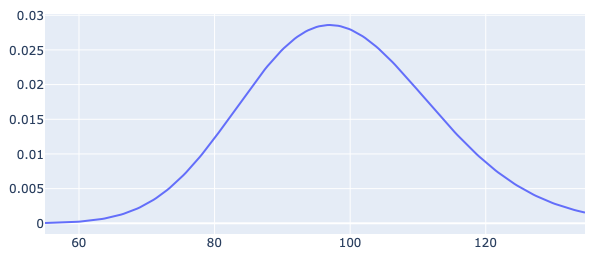
\includegraphics[width=0.8\textwidth]{distribution}
	\caption{Approximate distribution of the test statistic $\Lambda$ for a likelihood ratio test. Under the null hypothesis, $\Lambda \dot\sim \chi^{2}_{99}$.}
\end{figure}

    
    \hypertarget{f-determine-the-rejection-region-at-a-significance-level-of-0.05.-depict-it-in-the-previous-plot.}{%
\subparagraph{(f) Determine the rejection region at a significance level
of 0.05. Depict it in the previous
plot.\\[2ex]}\label{f-determine-the-rejection-region-at-a-significance-level-of-0.05.-depict-it-in-the-previous-plot.}}

    In this case, the rejection threshold is given by:

\begin{figure}[H]
	\centering
	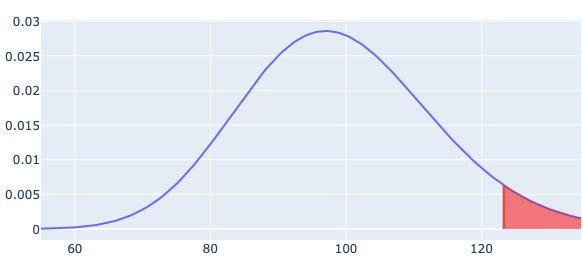
\includegraphics[width=0.8\textwidth]{rejectionRegion1}
	\caption{Rejection region (red) for the likelihood ratio test with significance level $\alpha = 0.05$.}
\end{figure}

    
    
    \hypertarget{g-also-show-the-value-of-the-test-statistic-in-the-previous-plot.-what-is-its-p-value-based-on-the-data-collected-by-the-observatory-and-the-analysis-that-you-have-conducted-does-the-emission-rate-appear-to-be-constant}{%
\subparagraph{\texorpdfstring{(g) Also show the value of the test
statistic in the previous plot. What is its \(p\)-value? Based on the
data collected by the observatory and the analysis that you have
conducted, does the emission rate appear to be
constant?\\[2ex]}{(g) Also show the value of the test statistic in the previous plot. What is its p-value? Based on the data collected by the observatory and the analysis that you have conducted, does the emission rate appear to be constant?}}\label{g-also-show-the-value-of-the-test-statistic-in-the-previous-plot.-what-is-its-p-value-based-on-the-data-collected-by-the-observatory-and-the-analysis-that-you-have-conducted-does-the-emission-rate-appear-to-be-constant}}

    The value of the test statistic is \texttt{104.40},which in the previous plot falls outside the rejection region

\begin{figure}[H]
	\centering
	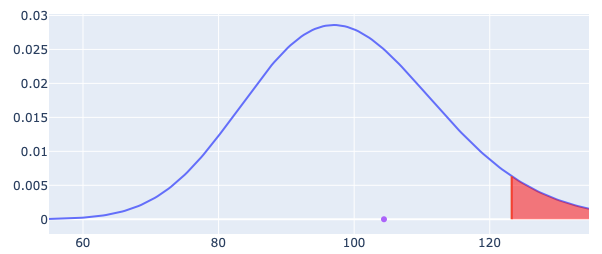
\includegraphics[width=0.8\textwidth]{notRejected}
	\caption{Rejection region (red) for the likelihood ratio test with significance level $\alpha = 0.05$. The value of the statistic $\Lambda$ is shown in the purple dot.}
\end{figure}
    
    The \(p\)-value associated with this value is \texttt{0.34}. Hence, under this assumptions, the null cannot be rejected and thus the emission rate appears to be constant.

    \hypertarget{problem-1.3-p-values}{%
\section*{\texorpdfstring{\textbf{Problem 1.3:}
\(p\)-values}{Problem 1.3: p-values}}\label{problem-1.3-p-values}}

Read the statement by the American Statistical Association about
\(p\)-values
(\href{https://github.com/pipeton8/6.439-stats-comp-applications/blob/main/Assignments/1\%20-\%20Stats\%20Review/The\%20ASA\%20s\%20Statement\%20on\%20p\%20Values\%20Context\%20Process\%20and\%20Purpose.pdf}{Wasserstein
and Lazar: The ASA's statement on p-values: context, process, and
purpose}) and respond to the following scenarios.

    \hypertarget{a-a-friend-looking-at-your-notes-from-the-first-lecture-saw-that-theres-a-p-value-of-0.0012-for-the-hip-study.-they-ask-you-does-that-mean-theres-a-99.88-chance-that-offering-a-mammography-decreases-the-risk-of-death-from-breast-cancer-explain-to-your-friend-exactly-what-this-p-value-means-including-any-assumptions-that-were-made.}{%
\subparagraph{\texorpdfstring{(a) A friend looking at your notes from
the first lecture saw that there's a \(p\)-value of 0.0012 for the HIP
study. They ask you, does that mean there's a 99.88\% chance that
offering a mammography decreases the risk of death from breast cancer?
Explain to your friend exactly what this \(p\)-value means, including
any assumptions that were
made.\\[2ex]}{(a) A friend looking at your notes from the first lecture saw that there's a p-value of 0.0012 for the HIP study. They ask you, does that mean there's a 99.88\% chance that offering a mammography decreases the risk of death from breast cancer? Explain to your friend exactly what this p-value means, including any assumptions that were made.}}\label{a-a-friend-looking-at-your-notes-from-the-first-lecture-saw-that-theres-a-p-value-of-0.0012-for-the-hip-study.-they-ask-you-does-that-mean-theres-a-99.88-chance-that-offering-a-mammography-decreases-the-risk-of-death-from-breast-cancer-explain-to-your-friend-exactly-what-this-p-value-means-including-any-assumptions-that-were-made.}}

    According to Wasserstein and Lazar (2016), for a certain statistical
model, the \(p\)-value is ``the probability (\ldots) that a statistical
summary of the data (\ldots) would be equal to or more extreme than its
observed value.'' In that sense, the interpretation of my friend is
incorrect. To understand what this \(p\)-value means, first note that the HIP was
based on two assumptions:
	\begin{itemize}
		\item That a person dying from breast cancer follows a Bernoulli distribution
with parameter \(\pi\).

		\item That a person dying from breast cancer is independent of other people
dying (or not) from breast cancer.
	\end{itemize}
	
Under that model, a randomized control trial was designed and the
participants assigned randomly to treatment and control groups. Only the
first were offered mammographies. The \(p\)-value in questions arises
when testing the (null) hypothesis that the probability of dying of
breast cancer (the \(\pi\) parameter of the Bernoulli distribution) is
the same for both groups. If that hypothesis were true, then a certain
test statistic (namely, the number of deaths in the treatment group)
follows a Hypergeometric distribution and the probability of the test
statistic being lower that the obtained value is 0.12\%. In other words,
there is a 99.88\% of probability that this statistical summary is
greater that its observed value. Additionally, it means there is at most
a probability of 0.12\% for the null hypothesis being true, although we
rejected it being so.

An additional (and hidden) assumption made to obtain that \(p\)-value is
that the number of deaths in the study was known beforehand.

    \hypertarget{b-your-colleague-in-education-studies-cares-about-what-can-improve-the-education-outcome-in-early-childhood.-he-thinks-the-ideal-planning-should-be-to-include-as-many-variables-as-possible-and-regress-childrens-educational-outcome-on-the-set.-then-we-select-the-variables-that-are-shown-to-be-statistically-significant-and-inform-the-policy-makers.-is-this-approach-likely-to-produce-the-intended-good-policies-what-other-approach-to-this-problem-could-you-suggest}{%
\subparagraph{(b) Your colleague in education studies cares about what
can improve the education outcome in early childhood. He thinks the
ideal planning should be to include as many variables as possible and
regress children's educational outcome on the set. Then we select the
variables that are shown to be statistically significant and inform the
policy makers. Is this approach likely to produce the intended good
policies? What other approach to this problem could you
suggest?\\[2ex]}\label{b-your-colleague-in-education-studies-cares-about-what-can-improve-the-education-outcome-in-early-childhood.-he-thinks-the-ideal-planning-should-be-to-include-as-many-variables-as-possible-and-regress-childrens-educational-outcome-on-the-set.-then-we-select-the-variables-that-are-shown-to-be-statistically-significant-and-inform-the-policy-makers.-is-this-approach-likely-to-produce-the-intended-good-policies-what-other-approach-to-this-problem-could-you-suggest}}

    There are multiple problems with this approach. First, given a certain
significance threshold it is highly likely to obtain significant results
if testing multiple hypothesis without correction. However, even if the
tests are corrected fro multiple hypothesis testing, other problems
arise. As mentioned in the Wasserstein and Lazar (2016), at least four
caveats can be mentioned for this approach:
\begin{enumerate}
\item The statistically significance of the variables is ``only a measure
about data in relation to a specified hypothetical explanation'', which
in this case is the coefficient of the variable not being zero. This is,
we have evidence to reject the idea that the variable in particular is
not helpful in linearly predicting the outcome, albeit there is no idea
of causality involved.

\item If we present the policymakers only the statistically significant
variables and do not report how the results were obtained, it is
impossible to draw clear and useful conclusions for policymaking. Like
the paper mentioned, \(p\)-values are uninterpretable in absence of the
models that produced them. After all, \(p\)-values are by definition
tied to a certain statistical model and assumptions.

\item The variable being statistically significant does not mean the effect it
could have on the outcome is big, or cost-effective to be a good public
policy. As mentioned by the authors: ``{[}s{]}maller \(p\)-values do not
necessarily imply the presence of larger or more important
effects(\ldots)''. In this case, finding a statistically significant
variable does not mean their effect on education is large enough to
become a good policy.

\item Finally, the statistical significance of the variables is not an
indicator of the underlying model being right. This, because the test
was realized assuming the model was right. In other words, testing
whether a variable is statistically significant in a certain model is
not a test about the model assumptions. Wasserstein and Lazar (2016)
elaborate on this mentioning that ``{[}b{]}y itself, a \(p\)-value does
not provide a good measure of evidence regarding a model or
hypothesis.'' Since we are only testing one of the infinite possible
hypothesis, there is a chance another completely different model or
hypothesis could explain better the data we have.
\end{enumerate}

In light of these problems, a better framework could be combining
statistical methods with experiment design improvements. First, and
drawing from the paper, we could combine testing for significance with
confidence intervals, likelihood ratios or Bayesian methods. We could
also incorporate decision-theoretic modeling and false discovery rates.
This way, we could deviate our attention from testing and focus on the
estimation and the size of the effects that each feature has on the
outcome. Another approach would be designing good RCTs that could shed
more light on the effects that some variables can have on education.
Evidently, this is a long and costly process and should be done with
most caution and care, in order to draw correct conclusions and avoid
bias.

    \hypertarget{c-an-economist-collects-data-on-many-nationwide-variables-and-surprisingly-finds-that-if-she-runs-a-regression-between-chocolate-consumption-and-number-of-nobel-prize-laureates-the-coefficient-is-statistically-significant.-should-she-conclude-that-there-exists-a-relationship-between-nobel-prize-and-chocolate-consumption-explain-why.}{%
\subparagraph{(c) An economist collects data on many nationwide
variables and surprisingly finds that if she runs a regression between
chocolate consumption and number of Nobel prize laureates, the
coefficient is statistically significant. Should she conclude that there
exists a relationship between Nobel prize and chocolate consumption?
Explain
why.\\[2ex]}\label{c-an-economist-collects-data-on-many-nationwide-variables-and-surprisingly-finds-that-if-she-runs-a-regression-between-chocolate-consumption-and-number-of-nobel-prize-laureates-the-coefficient-is-statistically-significant.-should-she-conclude-that-there-exists-a-relationship-between-nobel-prize-and-chocolate-consumption-explain-why.}}

    As mentioned in caveat 1 of the previous question, the fact that the
coefficient is statistically significant only means that chocolate
consumption is useful at predicting the number of Nobel prize laureates.
However, no relationship is elicited this way. There could be other
variables not taken into account like investment on science or research
in general, quality of schools and universities, easiness of migration,
among others, that could explain better the number of Nobel prize
laureates by country.

    \hypertarget{d-your-lab-collects-individual-level-data-on-50000-humans-for-100-features-including-iq-and-chocolate-consumption.-they-find-that-their-initial-hypothesis-about-the-relation-between-chocolate-consumption-and-iq-has-a-p-value-higher-than-0.05.-however-they-find-that-there-are-other-variables-in-the-data-set-that-have-p-value-less-than-0.05-namely-a-subjects-family-income-and-number-of-siblings.-they-therefore-decide-to-not-write-about-chocolate-consumption-but-rather-report-these-statistically-significant-results-in-their-paper-and-provide-possible-explanations.-is-this-sound-scientific-practice-please-discuss.}{%
\subparagraph{\texorpdfstring{(d) Your lab collects individual-level
data on 50,000 humans for 100 features, including IQ and chocolate
consumption. They find that their initial hypothesis about the relation
between chocolate consumption and IQ has a \(p\)-value higher than 0.05.
However, they find that there are other variables in the data set that
have p-value less than 0.05, namely, a subject's family income and
number of siblings. They therefore decide to not write about chocolate
consumption, but rather, report these statistically significant results
in their paper, and provide possible explanations. Is this sound
scientific practice? Please
discuss.\\[2ex]}{(d) Your lab collects individual-level data on 50,000 humans for 100 features, including IQ and chocolate consumption. They find that their initial hypothesis about the relation between chocolate consumption and IQ has a p-value higher than 0.05. However, they find that there are other variables in the data set that have p-value less than 0.05, namely, a subject's family income and number of siblings. They therefore decide to not write about chocolate consumption, but rather, report these statistically significant results in their paper, and provide possible explanations. Is this sound scientific practice? Please discuss.}}\label{d-your-lab-collects-individual-level-data-on-50000-humans-for-100-features-including-iq-and-chocolate-consumption.-they-find-that-their-initial-hypothesis-about-the-relation-between-chocolate-consumption-and-iq-has-a-p-value-higher-than-0.05.-however-they-find-that-there-are-other-variables-in-the-data-set-that-have-p-value-less-than-0.05-namely-a-subjects-family-income-and-number-of-siblings.-they-therefore-decide-to-not-write-about-chocolate-consumption-but-rather-report-these-statistically-significant-results-in-their-paper-and-provide-possible-explanations.-is-this-sound-scientific-practice-please-discuss.}}

    Exploratory studies may prove useful to discover suggestive
relationships in the data. However, these are not meant to be conclusive
about relationships between outcome variables and possible predictors.
As mentioned before, if 100 features are tested then, in average, under
a 0.05 significance threshold we should expect to find around 5
variables to be statistically significant, just by chance alone. This
can happen even if we correct our \(p\)-values for multiple hypothesis
testing. Consequently, this is not an ethical way to produce scientific
knowledge, less make decisions based on these discoveries.

The adequate way to move forward after an exploratory analysis is
finding good experiments (like RCTs or natural experiments) that could
allow us to test independently these hypotheses. Afterwards, we could
also provide explanations and try to test whether these are consistent
with the data.

    \hypertarget{e-a-neuroscience-lab-runs-a-randomized-experiment-on-100-mice-by-adding-chocolate-in-half-of-the-mices-diet-and-another-food-of-the-equivalent-calories-in-another-halfs-diet.-they-find-that-the-difference-between-the-two-groups-time-in-solving-a-maze-puzzle-has-a-p-value-lower-than-0.05.-should-they-conclude-that-chocolate-consumption-leads-to-improved-cognitive-power-in-mice-explain-why.}{%
\subparagraph{\texorpdfstring{(e) A neuroscience lab runs a randomized
experiment on 100 mice by adding chocolate in half of the mice's diet
and another food of the equivalent calories in another half's diet. They
find that the difference between the two groups' time in solving a maze
puzzle has a \(p\)-value lower than 0.05. Should they conclude that
chocolate consumption leads to improved cognitive power in mice? Explain
why.\\[2ex]}{(e) A neuroscience lab runs a randomized experiment on 100 mice by adding chocolate in half of the mice's diet and another food of the equivalent calories in another half's diet. They find that the difference between the two groups' time in solving a maze puzzle has a p-value lower than 0.05. Should they conclude that chocolate consumption leads to improved cognitive power in mice? Explain why.}}\label{e-a-neuroscience-lab-runs-a-randomized-experiment-on-100-mice-by-adding-chocolate-in-half-of-the-mices-diet-and-another-food-of-the-equivalent-calories-in-another-halfs-diet.-they-find-that-the-difference-between-the-two-groups-time-in-solving-a-maze-puzzle-has-a-p-value-lower-than-0.05.-should-they-conclude-that-chocolate-consumption-leads-to-improved-cognitive-power-in-mice-explain-why.}}

    This may not be a right conclusion to make after this experiment. Note
that, since this is a randomized experiment, the problem in this case is
not its statistical design, but in its conclusions. Strictly speaking,
they just proved that replacing half of the diet of the mice with
chocolate improved their maze solving time but not necessarily their
skills. There may be other explanations for this difference that are not
the mice improving their cognitive skills.

For example, since chocolate contains sugar, then is natural that mice
are more active (e.g.~run faster) and thus take less time than their
counterparts that did not have a diet change. In order to test an
improved cognitive power there should be used test that rely less on
time and more on other expression of cognition.

    \hypertarget{problem-1.4-published-research-findings-are-false}{%
\section*{\texorpdfstring{\textbf{Problem 1.4:} Published research
findings are
false}{Problem 1.4: Published research findings are false}}\label{problem-1.4-published-research-findings-are-false}}

Read the
\href{https://github.com/pipeton8/6.439-stats-comp-applications/blob/main/Assignments/1\%20-\%20Stats\%20Review/Ioannidis_paper.pdf}{paper
by Ioannidis (PLoS Medicine, 2005)} on why most published research
findings are false and summarize the paper in your own words.\\[2ex] {\bf What is
the most important lesson you learned from reading this paper? Explain
the computations going into Table 1, Table 2, and Table 3. How does
Ioannidis get to the conclusion that a research finding is more likely
true than false if $(1 - \beta)R \textgreater{} \alpha $ (at the
beginning of page 697)? What does this mean?}

    The author proposes a simple theoretical framework to explain why many
research findings in science could in principle be false. The three
models Ioannidis proposes focus primarily on three parameters:
\begin{itemize}
\item \(R\), the fraction of ``true relationships'' to ``no relationships''
among the relationships tested in a given field. From this, he computes
the pre-study (ex ante) probability of a relationship taken at random
being true: \(\frac{R}{R+1}\).

\item \(\alpha\), the significance threshold (i.e., the probability of
claiming the existence of a relationship where is none).

\item \(\beta\), the statistical power of the study (i.e., the probability of
finding a true relationship).
\end{itemize}

In his first model, the author compares in a contingency table (Table 1
in the paper) the expected number of studies that belong to each of the
4 groups given by: finding or rejecting a relationship, and the actual
existence (or not) of a relationship. Under this simple model is that he
proposes that a research finding is more likely true than false if
\((1-\beta)R > \alpha\).

This arises from the following calculation. If \(c\) studies are
conducted in a field, then a fraction \((1-\beta)\frac{R}{R+1}\) of them
are true findings (computed as the probability of finding a true
relationship times the probability of that finding being true). Also, a
fraction \(\alpha\frac{1}{R+1}\) of the studies are false research
findings (computed as the probability of falsely claiming a finding
times the probability of not being in presence of a relationship).
Consequently, a fraction \(\frac{\alpha + (1-\beta)R}{R+1}\) of the
studies are research findings (the sum of both previous ratios), and if
one is taken at random, its more likely to be true than false if and
only if the fraction of true findings is greater than the fraction of
false findings: \[\frac{(1-\beta)R}{R+1} > \frac{\alpha}{R+1}\] which
translates to \((1-\beta)R > \alpha\). This condition is equivalent to
the positive predictive value (PPV) being greater than 0.5, where
\[ PPV = \frac{\text{fraction of true research findings}}{\text{fraction of research findings}} = \frac{\frac{(1-\beta)R}{R+1}}{\frac{\alpha + (1-\beta)R}{R+1}} = \frac{(1-\beta)R}{\alpha + (1-\beta)R} \]
Indeed,
\[PPV > 0.5 \Longleftrightarrow (1-\beta)R > 0.5\alpha + 0.5(1-\beta)R \Longleftrightarrow (1-\beta)R > \alpha \]
Note that the PPV is nothing more than the ex post probability of a
relationship being true. Hence, the Ioannidis' claim translates to: we
could expect that a given research finding is more likely false than
true if the probability of being true, after being tested is
strictly greater than a 50\%. Of course, we could aim for a more strict
threshold, but 50\% is the minimum necessary to make the appearance of
true findings more likely.

Later in the paper the author makes more complex assumptions and
incorporates, separately, two variations:
\begin{enumerate}
\item Presence of bias, that is, the probability that a given study was passed
as a research finding, although there was none.

\item Presence of multiple independent studies, that is, the fact that many
independent research teams are testing the same relationship
simultaneously.
\end{enumerate}

These new models are summarized in Tables 2 and 3, respectively. These
tables follow the same logic as the first one, where studies are split
in four groups and the expected values computed based on the
probabilities of belonging to each group, now including bias and multiple
independent testing.

The main contribution of the paper is showing using a very simple
framework that finding true relationships from published research
findings is not as probable as we may expect. Moreover, the author shows
to how extent different aspects of the studies are affecting the ex post
probability of the finding being true. In this line, Ioannidis shows
that the ex ante probability is one of the main drivers of the veracity
of research findings. Statistical power and bias also have a important
effect. In his closing remarks, the author provides at least three
solutions: better evidence (e.g.~large-scale studies in relationships
with high ex ante probability of being true), pre-register studies to
reduce bias (or at least adhering to a scientific protocol), and better
understand the range of \(R\) values for each field (and promote fields
where \(R\) is bigger).

In that sense, the lesson I learned from the paper is that we have to be
very critical when interpreting results from studies. Biased fields can
have many false results posing as true, especially if the study design
did not achieve high power. The same can be said about questions that
draw a lot of attention from the scientific and social community, in
particular those that fight to produce a highly significant or strong
result (although there may be none). For example, due to the pandemic a
lot of interest was drawn towards questions about the effects that some
policies could have on the pandemic control or the effects than the
pandemic can have in different aspects of our lives. It is possible that
the \(R\) value for this field may be large (as there are a lot we do
not know yet on pandemics), but there may also be a lot of bias in which
relationships want to be answered and which pre conceived answers are
expected. Moreover, many teams are tackling simultaneously similar
questions, which as mentioned can produce false results. Last but not
least, there is possible that for these questions is not possible to
design good experiments and we must have to relay on natural experiments
or country-or-state-level quasi-experiments, which have much less
power.\\
    
\newpage
    \hypertarget{problem-1.5-detecting-leukemia-types}{%
\section*{\texorpdfstring{\textbf{Problem 1.5:} Detecting Leukemia
types}{Problem 1.5: Detecting Leukemia types}}\label{problem-1.5-detecting-leukemia-types}}

The data set \texttt{golub}\footnote{\textbf{Source of data:} Golub et al.~(1999).
\href{https://www.science.org/doi/10.1126/science.286.5439.531?url_ver=Z39.88-2003\&rfr_id=ori:rid:crossref.org\&rfr_dat=cr_pub\%20\%200pubmed}{\emph{Molecular
classification of cancer: class discovery and class prediction by gene
expression monitoring}}, Science, Vol. 286:531-537.} consists of the expression levels of 3,051
genes for 38 tumor mRNA samples. Each tumor mRNA sample comes from one
patient (i.e., 38 patients total): 27 of these tumor samples correspond
to acute lymphoblastic leukemia (ALL), while the remaining 11 correspond
to acute myeloid leukemia (AML).\\[1ex]

{\bf How many genes are associated with the
different tumor types (meaning that their expression level differs
between the two tumor types) using (i) the uncorrected \(p\)-values,
(ii) the Holm-Bonferroni corrected \(p\)-values, and (iii) the
Benjamini-Hochberg corrected \(p\)-values? Feel free to use existing
libraries for multiple hypothesis testing, in \texttt{R} or
\texttt{python}. You can use \(\alpha = 0.05\) for the significance
threshold.}

    In order to determine which genes had different expression leves between
the two tumor types, for each gene a \(t\) test of means between each
group was performed. This test has a null hypothesis that both ALL and
AML samples have the same mean, against the alternative hypothesis that
the means are different. This test is equivalent to estimating, for each
gene \(g\), the linear model
\[y_{gi} = \beta_{g0} + \beta_{g1}\text{tumor}_{gi} + \varepsilon_{gi},\]
where \(y_gi\) is the expression level for gene \(g\) in patient \(i\),
and \(\text{tumor}_{gi}\) is the tumor class for sample \(i\) of gene
\(g\). Here, the null hypothesis \(\beta_{g1} = 0\) against
\(\beta_{g1} \neq 0\) is equivalent to the mean \(t\)-test.

For more robustness, the test was made without the assumption that
variances across groups are equal. The results are as follows:

\begin{itemize}
	\item Number of relevant genes without correction: 1078.

	\item Number of relevant genes using the Holm-Bonferroni correction: 103.

	\item Number of relevant genes using the Benjamini-Hochberg correction: 695.
\end{itemize}

As expected, the Holm-Bonferroni correction is the most conservative, as
it tries to minimize the FWER. The Benjamini-Hochberg is less
conservative, categorizing almost 35\% of the rejected hypothesis as
false discoveries.

\newpage
    \hypertarget{problem-1.6-regression-and-gradient-descent}{%
\section*{\texorpdfstring{\textbf{Problem 1.6:} Regression and
Gradient
Descent}{Problem 1.6: Regression and Gradient Descent}}\label{problem-1.6-regression-and-gradient-descent}}

In this problem, we will look at OLS and the gradient descent algorithm.

    \hypertarget{a-read-in-the-synthetic-data-matrix-syn_x.csv-and-the-vector-syn_y.csv-of-observations.-compute-the-ols-estimator-hatbeta-by-matrix-inversion.}{%
\subparagraph{\texorpdfstring{(a) Read in the synthetic data matrix
\texttt{syn\_X.csv} and the vector \texttt{syn\_y.csv} of
``observations''. Compute the OLS estimator \(\hat{\beta}\) by matrix
inversion.\\[2ex]}{(a) Read in the synthetic data matrix syn\_X.csv and the vector syn\_y.csv of ``observations''. Compute the OLS estimator \textbackslash hat\{\textbackslash beta\} by matrix inversion.}}\label{a-read-in-the-synthetic-data-matrix-syn_x.csv-and-the-vector-syn_y.csv-of-observations.-compute-the-ols-estimator-hatbeta-by-matrix-inversion.}}

    The OLS estimator \(\hat{\beta}\) is obtained from the following
formula: 
	\[\hat{\beta} = \left(X^T X \right)^{-1} X^T y\]

In this case
	\[\hat{\beta} = \begin{pmatrix} 1.45 \\ -4.75\end{pmatrix}\]

\subparagraph{(b) Implement gradient descent for the least squares problem and run it on the synthetic test data loaded in the previous question. As a function of the iteration $t$, plot the mean squared error (MSE) and the distance $\|\beta^{t} - \hat{\beta}\|$ of your current iterates (in separate plots). Play with different initializations $\beta^{0}$ and different step sizes. What do you observe? Explain. Based on your observations, what would be an optimal step size?\\[2ex]}

As expected, the closer the initial $\beta_{0}$ is from $\hat{\beta}$, the faster the algorithm converges to it. In the figure below, the faster convergence happened with $\beta_0 = \begin{pmatrix} 2 \\ -1 \end{pmatrix}$, which is extremely close o $\hat{\beta}$ computed before.

\begin{figure}[H]
	\centering
	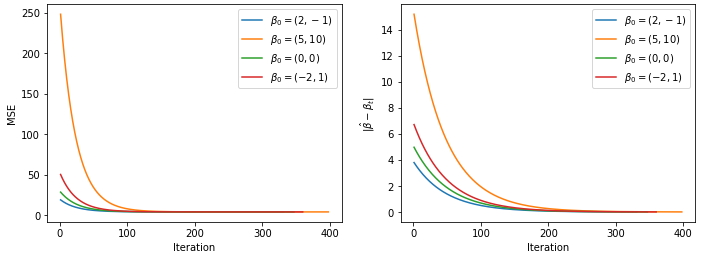
\includegraphics[width=0.85\textwidth]{GD_iterations_beta0}
	\caption{MSE and distance to true estimate for different initial vectors $\beta_{0}$. Step size = 0.01.}
\end{figure}


In terms of step sizes, smallest values take more iterations to
converge. However, values close to 1 have problems converging, because
gradients tend to explode. In the figure below, a step size of 0.7 gave
the fastest convergence, but albeit a very steep one. On the other hand,
the value of 0.01 gave a slower convergence but more controlled. All in
all, it appears that an optimal value could be 0.05 or lower, in order
to prevent numerical instabilities.

\begin{figure}[H]
	\centering
	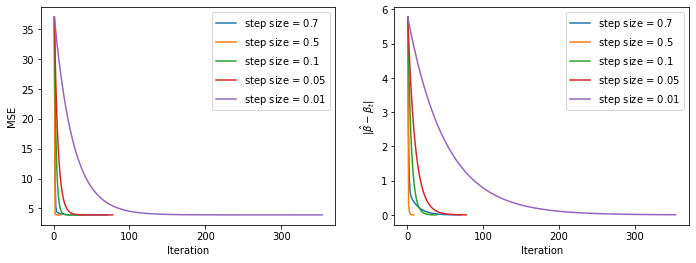
\includegraphics[width=0.85\textwidth]{GD_iterations_stepsize}
	\caption{MSE and distance to true estimate for different step size. Initial vector $\beta_{0} = (1,1)$.}
\end{figure}


   
    \hypertarget{next-we-look-at-some-real-data.-general-motors-collected-data-found-in-mortality.csv-from-60-us-cities-to-study-the-contribution-of-air-pollution-to-mortality.-the-dependent-variable-is-the-age-adjusted-mortality-mortality.-the-data-include-variables-measuring-climate-characteristics-jantemp-julytemp-relhum-rain-variables-measuring-demographic-characteristics-of-the-cities-educ-dens-nonwhite-whitecollar-pop-house-income-and-variables-recording-the-pollution-potential-of-three-different-air-pollutants-hc-nox-so2.}{%
\subparagraph{\texorpdfstring{Next, we look at some real data. General
Motors collected data (found in \texttt{mortality.csv}) from 60 US
cities to study the contribution of air pollution to mortality. The
dependent variable is the age-adjusted mortality (\texttt{Mortality}).
The data include variables measuring climate characteristics
(\texttt{JanTemp}, \texttt{JulyTemp}, \texttt{RelHum}, \texttt{Rain}),
variables measuring demographic characteristics of the cities
(\texttt{Educ}, \texttt{Dens}, \texttt{NonWhite}, \texttt{WhiteCollar},
\texttt{Pop}, \texttt{House}, \texttt{Income}), and variables recording
the pollution potential of three different air pollutants (\texttt{HC},
\texttt{NOx},
\texttt{SO2}).}{Next, we look at some real data. General Motors collected data (found in mortality.csv) from 60 US cities to study the contribution of air pollution to mortality. The dependent variable is the age-adjusted mortality (Mortality). The data include variables measuring climate characteristics (JanTemp, JulyTemp, RelHum, Rain), variables measuring demographic characteristics of the cities (Educ, Dens, NonWhite, WhiteCollar, Pop, House, Income), and variables recording the pollution potential of three different air pollutants (HC, NOx, SO2).\\[2ex]}}\label{next-we-look-at-some-real-data.-general-motors-collected-data-found-in-mortality.csv-from-60-us-cities-to-study-the-contribution-of-air-pollution-to-mortality.-the-dependent-variable-is-the-age-adjusted-mortality-mortality.-the-data-include-variables-measuring-climate-characteristics-jantemp-julytemp-relhum-rain-variables-measuring-demographic-characteristics-of-the-cities-educ-dens-nonwhite-whitecollar-pop-house-income-and-variables-recording-the-pollution-potential-of-three-different-air-pollutants-hc-nox-so2.}}

    \hypertarget{c-get-an-overview-of-the-data-and-account-for-possible-problems.-which-cities-stand-out-which-of-the-variables-need-to-be-transformed-when-applicable-which-transformations-would-you-apply}{%
\subparagraph{(c) Get an overview of the data and account for possible
problems. Which cities stand out? Which of the variables need to be
transformed? When applicable, which transformations would you
apply?\\[2ex]}\label{c-get-an-overview-of-the-data-and-account-for-possible-problems.-which-cities-stand-out-which-of-the-variables-need-to-be-transformed-when-applicable-which-transformations-would-you-apply}}

    One the first problems with the data is the lack of descriptions over
the variables. Even if statistical assumptions hold and the other
problems (I will mention below) are not present, it is impossible to
interpret quantitatively the results obtained.

Nevertheless, there are potential problems with the data that may bias
our results. First of all, looking at the population chart, is clear
that two cities are considerable bigger than the others: New York and
Los Angeles (see \Cref{fig:popchart}). 

\begin{figure}[H]
	\centering
	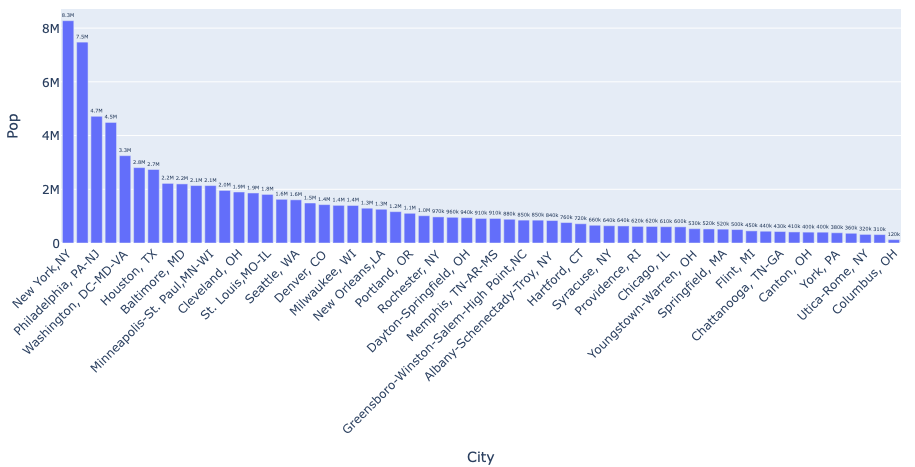
\includegraphics[width=0.7\textwidth]{pop_chart}
	\caption{Population chart of different cities in the database. Some cities with smaller populations are omitted.}
	\label{fig:popchart}
\end{figure}


Something similar happens when looking at the \texttt{HC}
and \texttt{NOx} variables, where Los Angeles and San Francisco stand
out from the others (see \Cref{fig:HC,fig:NOx}, respectively).

\begin{figure}[H]
	\begin{subfigure}[b]{\textwidth}
         \centering
         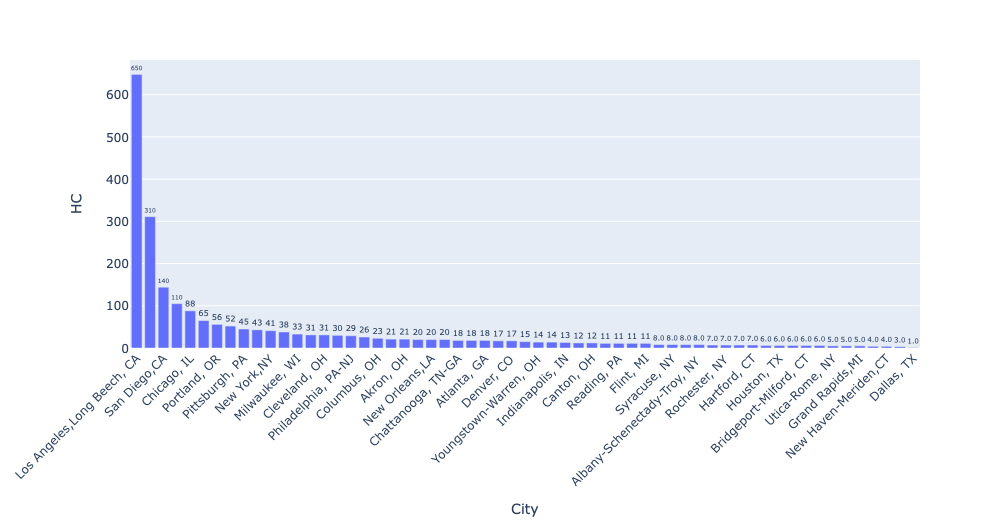
\includegraphics[width=\textwidth]{HC_chart}
         \caption{HC}
         \label{fig:HC}
    \end{subfigure}
    
	\begin{subfigure}[b]{\textwidth}
         \centering
         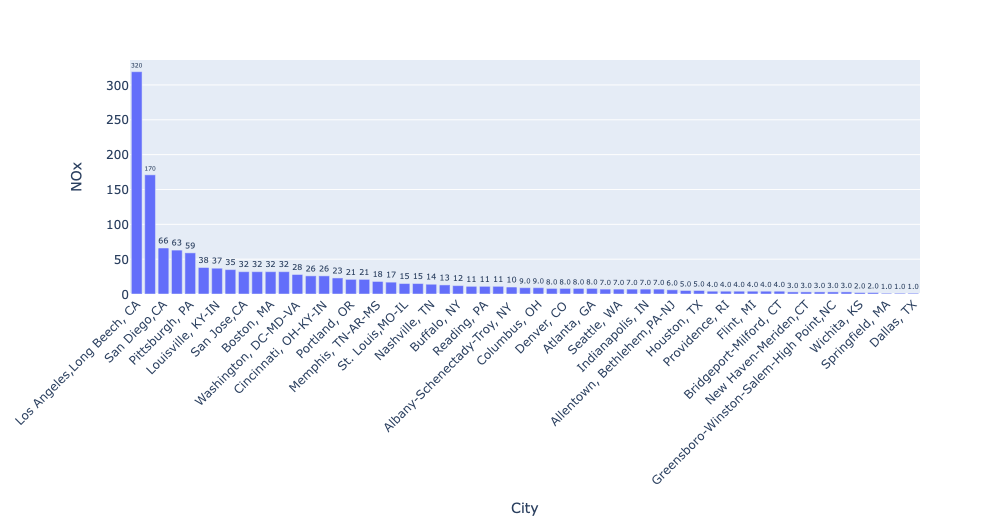
\includegraphics[width=\textwidth]{NOx_chart}
         \caption{$\text{NO}_{\text{x}}$}
         \label{fig:NOx}
    \end{subfigure}
	\caption{Pollutants chart of different cities in the database. Some cities with smaller values of pollutants are omitted.}
\end{figure}


Another potential issue with the data is that \texttt{HC} and
\texttt{NOx} are highly correlated (see \Cref{fig:correl}), with a Pearson correlation of 0.98). This may be due to cars or coal plants emitting both HC and NO$_{\text{x}}$ contaminants in a similar fashion. In order to estimate the effect of contaminants
over mortality, only one of these two variables should be included in
the regression model.

\begin{figure}[H]
	\centering
	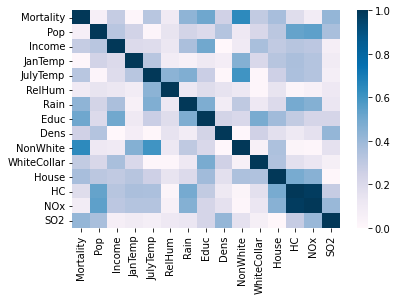
\includegraphics[width=0.6\textwidth]{correlMatrix}
	\caption{Matrix of absolute values of Pearson correlation coefficients, for the numeric variables in the dataset. A darker color implies a higher correlation.}
\end{figure}


Finally, the pair grid between \texttt{Mortality} and other control
variables does not present visual evidence that the latter need to be
transformed in order to include them in a regression model. However, to
avoid scale issues, variables \texttt{Pop} and \texttt{Income} could be
normalized to million of people and thousands of dollars, respectively.

\begin{figure}[H]
	\centering
	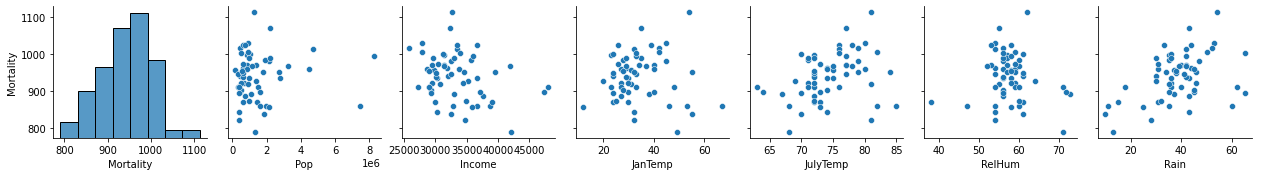
\includegraphics[width=\textwidth]{pairGrid1}
	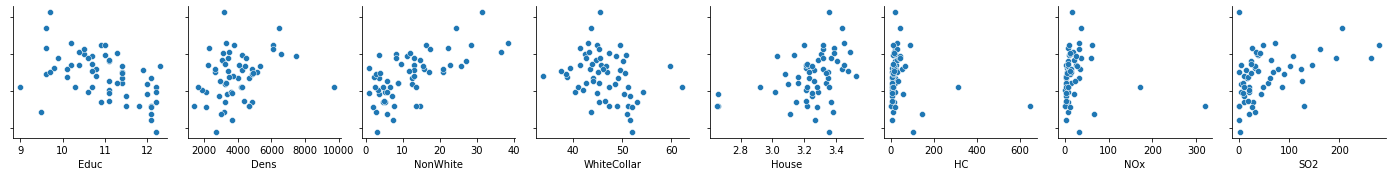
\includegraphics[width=\textwidth]{pairGrid2}	
	\caption{Pair grid for mortality and its potential predictors. The first graph is the histogram of \texttt{Mortality} and the others are scatterplots with \texttt{Mortality} as dependent variable and the corresponding independent variable indicated on the $X$ axis of each graph.}
\end{figure}


    
    \hypertarget{d-run-your-gradient-descent-algorithm-for-least-squares-on-the-raw-data-and-on-the-transformed-data-with-different-step-sizes-as-before.-what-do-you-observe}{%
\subparagraph{(d) Run your gradient descent algorithm for least squares
on the raw data and on the transformed data, with different step sizes
as before. What do you
observe?\\[2ex]}\label{d-run-your-gradient-descent-algorithm-for-least-squares-on-the-raw-data-and-on-the-transformed-data-with-different-step-sizes-as-before.-what-do-you-observe}}

    The GD algorithm applied in the raw data does not converge. This is most
likely happening due to numerical instability issues driven by the
variables with large numbers or the highly correlated variables
\texttt{HC} and \texttt{NOx}.

On the other hand, the algorithm converges for the transformed data,
albeit with a step size several orders of magnitude smaller than the
ones used in the previous exercise. For this reason, only one experiment
with step size equal to \(10^{-8}\) was performed. The most likely
explanation for this could be numerical issues driven by the different
units the variables are expressed in. Additionally, this could be due to
the presence of the outliers mentioned before. In order to induce the
convergence of the algorithm in less iterations, we would need to
normalize the variables (using standarization or min-max normalization)
and dropping the outliers, if necessary.
   
    \hypertarget{e-carry-out-a-multiple-linear-regression-containing-all-variables-with-the-necessary-transformations-with-gradient-descent-as-in-d-or-with-matrix-inversion.-does-the-model-fit-well-check-the-residuals-and-comment-on-what-you-observe.}{%
\subparagraph{(e) Carry out a multiple linear regression containing all
variables with the necessary transformations (with gradient descent as
in d) or with matrix inversion). Does the model fit well? Check the
residuals and comment on what you
observe.\\[2ex]}\label{e-carry-out-a-multiple-linear-regression-containing-all-variables-with-the-necessary-transformations-with-gradient-descent-as-in-d-or-with-matrix-inversion.-does-the-model-fit-well-check-the-residuals-and-comment-on-what-you-observe.}}

    After fitting the model (with a constant), the goodness-of-fit, given by the \(R^2\)
coefficient is almost 1, which is close to a perfect prediction for all
the data points in the sample. This is also confirmed by the residuals,
with magnitudes of \(10^{-9}\). However, by looking at \Cref{fig:residuals}, the residual plot evidences a trend, with lower errors for cities with large mortality and higher errors for cities with low mortality.
	
\begin{figure}[H]
	\centering
	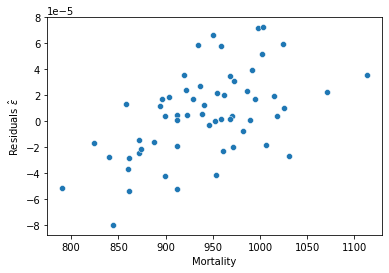
\includegraphics[width=0.6\textwidth]{residuals}
	\caption{Residuals of the regression model fitted on Mortality against all other numeric variables in the database.}
\end{figure}
	
The first problem could be related to a violation of the assumptions on
the normality of the error. There could be omitted variables that could
explain the mortality that we are not including in the model. Regarding
the second issue, the problem could be the prescence of outlier cities.
For these cities, a certain margin of error reuslts in a greater
increase in the loss function for them than for others with lower
mortality overall. This may induce the model to predict better the
mortality of those cities.
    
    \hypertarget{f-gradient-descent-for-other-functions-a-popular-regression-model-for-binary-observations-y-is-given-by-the-following-estimator-hatbeta-argmin_beta-sum_i-logleft1-expleft-y_i-betat-x_i-rightright-how-would-you-solve-this-via-gradient-descent-derive-the-corresponding-gradient-and-write-down-the-steps-of-the-algorithm.}{%
\subparagraph{\texorpdfstring{(f) \emph{Gradient descent for other
functions:} A popular regression model for binary observations \(y\) is
given by the following estimator:
\[ \hat{\beta} = \arg\min_{\beta} \sum_{i} \log\left(1 + \exp\left(-y_i \beta^T x_i \right)\right)\]
How would you solve this via gradient descent? Derive the corresponding
gradient and write down the steps of the
algorithm.\\[2ex]}{(f) Gradient descent for other functions: A popular regression model for binary observations y is given by the following estimator:  \textbackslash hat\{\textbackslash beta\} = \textbackslash arg\textbackslash min\_\{\textbackslash beta\} \textbackslash sum\_\{i\} \textbackslash log\textbackslash left(1 + \textbackslash exp\textbackslash left(-y\_i \textbackslash beta\^{}T x\_i~\textbackslash right)\textbackslash right) How would you solve this via gradient descent? Derive the corresponding gradient and write down the steps of the algorithm.}}\label{f-gradient-descent-for-other-functions-a-popular-regression-model-for-binary-observations-y-is-given-by-the-following-estimator-hatbeta-argmin_beta-sum_i-logleft1-expleft-y_i-betat-x_i-rightright-how-would-you-solve-this-via-gradient-descent-derive-the-corresponding-gradient-and-write-down-the-steps-of-the-algorithm.}}

    First, note that \(\log\) is a non-decreasing convex function, and
\(1 + \exp(w)\) is convex. Hence, each of the terms in the summation are
convex and the loss function is convex as well. This implies that the
gradient descent algorithm will converge, given an adequate step size.

Now, in order to describe the algorithm we need to compute the gradient
of this loss function. Let \(L(\beta)\) be the loss function. Then
\[\frac{\partial L}{\partial \beta_j} = \sum_i -y_i x_{ij}\frac{\exp\left(-y_i \beta^T x_i\right)}{1 + \exp\left(-y_i \beta^T x_i\right)}\]

Consequently, for step size \(\alpha\), the update of the algorithm for
coordinate \(j\) of iteration \(\beta_t\) is
\[\beta_{t+1,j} \leftarrow \beta_{t,j} - \alpha \frac{\partial L}{\partial \beta_j}\]

    \hypertarget{problem-1.7-computational-aspects-of-regression}{%
\section*{\texorpdfstring{\textbf{Problem 1.7:} Computational Aspects
of
Regression}{Problem 1.7: Computational Aspects of Regression}}\label{problem-1.7-computational-aspects-of-regression}}

In this problem, we will consider some computational challenges that
arise in practice when performing linear regression.

    \hypertarget{a-suppose-you-have-a-problem-in-which-the-feature-matrix-x-has-100-million-rows-and-200-columns.-what-challenge-will-arise-when-you-try-to-apply-either-the-matrix-inversion-method-or-the-gradient-descent-method-to-compute-the-regression-coefficients-as-in-the-previous-problem-hint-if-each-entry-is-a-64-bit-float-how-much-memory-will-be-required-to-store-x}{%
\subparagraph{\texorpdfstring{(a) Suppose you have a problem in which
the feature matrix, \(X\), has 100 million rows and 200 columns. What
challenge will arise when you try to apply either the matrix inversion
method or the gradient descent method to compute the regression
coefficients as in the previous problem? \emph{Hint: if each entry is a
64-bit float, how much memory will be required to store
\(X\)?\\[2ex]}}{(a) Suppose you have a problem in which the feature matrix, X, has 100 million rows and 200 columns. What challenge will arise when you try to apply either the matrix inversion method or the gradient descent method to compute the regression coefficients as in the previous problem? Hint: if each entry is a 64-bit float, how much memory will be required to store X?}}\label{a-suppose-you-have-a-problem-in-which-the-feature-matrix-x-has-100-million-rows-and-200-columns.-what-challenge-will-arise-when-you-try-to-apply-either-the-matrix-inversion-method-or-the-gradient-descent-method-to-compute-the-regression-coefficients-as-in-the-previous-problem-hint-if-each-entry-is-a-64-bit-float-how-much-memory-will-be-required-to-store-x}}

    A matrix \(X\) of that size would have \(2 \cdot 10^{10}\) entries. If
every entry is a 64-bit float, then each entry needs 8 bytes of memory
to be stored. Consequently, to store the matrix \(X\) would be needed:
\[ \frac{2 \cdot 10^{10}}{10^{9}} = 20\, GB\] of memory. This, without
considering matrix additional matrix operations needed to invert \(X\)
or compute the gradient and the update of gradient descent algorithm.

Hence, for a problem like this we would need a different mechanism to
compute the regression coefficients.

    \hypertarget{b-suggest-one-method-that-will-allow-you-to-compute-the-linear-regression-coefficients-for-this-problem.-be-specific.-discuss-pros-and-cons-of-your-proposed-approach.}{%
\subparagraph{(b) Suggest one method that will allow you to compute the
linear regression coefficients for this problem. Be specific. Discuss
pros and cons of your proposed
approach.\\[2ex]}\label{b-suggest-one-method-that-will-allow-you-to-compute-the-linear-regression-coefficients-for-this-problem.-be-specific.-discuss-pros-and-cons-of-your-proposed-approach.}}

    An option would be to use the stochastic gradient descent (SGD)
algorithm. For this algorithm, we have the following steps:
\begin{enumerate}
	\item Define batch size \texttt{batch\_size}. Also define initial state
\(\beta_0\), initial loss function value \(L_0\) (large), step size
\(\alpha\) and tolerance \(\epsilon\) for the GD algorithm.

	\item Sample randomly \texttt{batch\_size} many numbers between 0 and 100
million (with replacement). Load the sampled rows of \(X\) (including
all columns) into dataset \texttt{df}.

	\item Compute gradient using \texttt{df} and update
\(\beta_t \to \beta_{t+1}\) using step\_size \(\alpha\).

	\item Compute loss function \(L_{t+1}\) with \(\beta_{t+1}\).

	\item If \(|L_{t+1} - L_{t}| \leq \epsilon\), define
\(\hat{\beta} = \beta_{t+1}\) and terminate. Otherwise, return to step
2.
\end{enumerate}

Assuming the loss function is convex, then SGD will converge given a
correctly specified step size, even if \texttt{batch\_size} is small. An
advantage of using SGD is that the process is much more efficient, even
if the necessary memory to run GD is available. However, it is possible
that SGD takes much more steps if the loss function is not smooth
enough.

    \hypertarget{now-suppose-we-are-in-a-setting-in-which-the-number-of-data-points-n-is-much-smaller-than-the-number-of-variables-p-i.e.-x-has-many-more-columns-than-rows.-this-situation-occurs-often-in-biological-applications-for-example-in-which-the-features-may-represent-the-expression-levels-of-various-genes.-this-is-often-referred-to-as-the-high-dimensional-regime.-assume-x-is-small-enough-that-it-can-fit-in-memory.}{%
\subparagraph{\texorpdfstring{Now, suppose we are in a setting in which
the number of data points, \(n\), is much smaller than the number of
variables, \(p\), i.e., \(X\) has many more columns than rows. This
situation occurs often in biological applications, for example, in which
the features may represent the expression levels of various genes. This
is often referred to as the ``high-dimensional'' regime. (Assume \(X\)
is small enough that it can fit in
memory.)}{Now, suppose we are in a setting in which the number of data points, n, is much smaller than the number of variables, p, i.e., X has many more columns than rows. This situation occurs often in biological applications, for example, in which the features may represent the expression levels of various genes. This is often referred to as the ``high-dimensional'' regime. (Assume X is small enough that it can fit in memory.)}}\label{now-suppose-we-are-in-a-setting-in-which-the-number-of-data-points-n-is-much-smaller-than-the-number-of-variables-p-i.e.-x-has-many-more-columns-than-rows.-this-situation-occurs-often-in-biological-applications-for-example-in-which-the-features-may-represent-the-expression-levels-of-various-genes.-this-is-often-referred-to-as-the-high-dimensional-regime.-assume-x-is-small-enough-that-it-can-fit-in-memory.}}

    \hypertarget{c-can-we-run-gradient-descent-to-compute-the-regression-coefficients-what-do-you-think-about-the-solution-why-hint-what-is-the-maximum-rank-of-the-matrix-xt-x}{%
\subparagraph{\texorpdfstring{(c) Can we run gradient descent to compute
the regression coefficients? What do you think about the solution? Why?
\emph{Hint: what is the maximum rank of the matrix
\(X^T X\)?\\[2ex]}}{(c) Can we run gradient descent to compute the regression coefficients? What do you think about the solution? Why? Hint: what is the maximum rank of the matrix X\^{}T X?}}\label{c-can-we-run-gradient-descent-to-compute-the-regression-coefficients-what-do-you-think-about-the-solution-why-hint-what-is-the-maximum-rank-of-the-matrix-xt-x}}

    In this setting, there are infinite solutions to the problem of
minimizing the MSE. In that sense, running GD on the MSE alone may not
converge. Moreover, even if it converges, the solution will vary between
different runs of the algorithm if the initial state or the step size
are changed. Consequently, there is no possible way of making
conclusions about the solution unless we impose some kind of
regularization.

    \hypertarget{d-load-the-data-from-the-previous-question-syn_x.csv-and-syn_y.csv.-compute-the-regression-coefficients-by-solving-the-lasso-problem-for-various-values-of-lambda.-what-happens-to-the-solution-as-lambda-increases-choose-lambda-such-that-only-one-component-of-the-coefficient-vector-is-nonzero.-what-is-the-value-of-lambda-which-coefficient-is-it-for-this-problem-feel-free-to-use-a-package-that-performs-lasso-regularization-such-as-scikit-learn-in-python-or-glmnet-in-r.}{%
\subparagraph{\texorpdfstring{(d) Load the data from the previous
question, \texttt{syn\_X.csv} and \texttt{syn\_Y.csv}. Compute the
regression coefficients by solving the LASSO problem for various values
of \(\lambda\). What happens to the solution as \(\lambda\) increases?
Choose \(\lambda\) such that only one component of the coefficient
vector is nonzero. What is the value of \(\lambda\)? Which coefficient
is it? (For this problem, feel free to use a package that performs LASSO
regularization, such as \texttt{scikit-learn} in \texttt{python} or
\texttt{glmnet} in
\texttt{R}.)\\[2ex]}{(d) Load the data from the previous question, syn\_X.csv and syn\_Y.csv. Compute the regression coefficients by solving the LASSO problem for various values of \textbackslash lambda. What happens to the solution as \textbackslash lambda increases? Choose \textbackslash lambda such that only one component of the coefficient vector is nonzero. What is the value of \textbackslash lambda? Which coefficient is it? (For this problem, feel free to use a package that performs LASSO regularization, such as scikit-learn in python or glmnet in R.)}}\label{d-load-the-data-from-the-previous-question-syn_x.csv-and-syn_y.csv.-compute-the-regression-coefficients-by-solving-the-lasso-problem-for-various-values-of-lambda.-what-happens-to-the-solution-as-lambda-increases-choose-lambda-such-that-only-one-component-of-the-coefficient-vector-is-nonzero.-what-is-the-value-of-lambda-which-coefficient-is-it-for-this-problem-feel-free-to-use-a-package-that-performs-lasso-regularization-such-as-scikit-learn-in-python-or-glmnet-in-r.}}

    The results are presented in \Cref{fig:evolutionLasso}. As \(\lambda\) increases, the size of the coefficient vector shrinks
towards 0 linearly. The first component to become zero is \(\beta_0\),
which achieves this value with \(\lambda = 1.81\). The second
coefficient becomes zero with \(\lambda = 4.67\).

\begin{figure}[H]
	\centering
	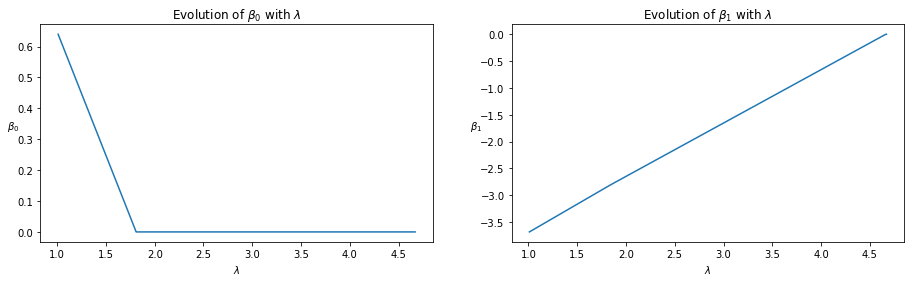
\includegraphics[width=\textwidth]{evolutionLasso}
	\caption{Evolution of each coefficient of linear regression \texttt{syn\_y} $=$ \texttt{syn\_X}$\beta + \varepsilon$ as a function of the Lasso parameter $\lambda$.}
\end{figure}

    
    \hypertarget{problem-1.8-likelihood-ratio-test-for-a-gaussian-model}{%
\section*{\texorpdfstring{\textbf{Problem 1.8:} Likelihood ratio test
for a Gaussian
model}{Problem 1.8: Likelihood ratio test for a Gaussian model}}\label{problem-1.8-likelihood-ratio-test-for-a-gaussian-model}}

In this problem, we will analyze the likelihood ratio statistic for the
model \(X \sim \mathcal{N}(\mu,\sigma^2)\) with unknown mean and unknown
variance and null hypothesis \(H_0 : \mu = 0\) versus alternative
hypothesis \(H_A : \mu \neq 0\).

    \hypertarget{a-what-is-the-likelihood-function-for-n-independent-and-identically-distributed-iid-gaussian-random-variables-with-mean-mu-and-variance-sigma2}{%
\subparagraph{\texorpdfstring{(a) What is the likelihood function for
\(n\) independent and identically distributed (iid) Gaussian random
variables (with mean \(\mu\) and variance
\(\sigma^2\))?}{(a) What is the likelihood function for n independent and identically distributed (iid) Gaussian random variables (with mean \textbackslash mu and variance \textbackslash sigma\^{}2)?}}\label{a-what-is-the-likelihood-function-for-n-independent-and-identically-distributed-iid-gaussian-random-variables-with-mean-mu-and-variance-sigma2}}

    The likelihood function for \(n\) iid Gaussian random variables with
mean \(\mu\) and variance \(\sigma^2\) is
\[p_{\mu, \sigma^2}(x_1, \ldots, x_n) = \prod_{i=1}^n \frac{1}{\sigma (2\pi)^{1/2}}\, \exp\left(\frac{1}{2\sigma^2}(x_i - \mu)^2\right) = \frac{1}{\sigma^n (2\pi)^{n/2}} \exp\left( \frac{1}{2\sigma^2} \sum_{i=1}^{n} (x_i- \mu)^2 \right) \]

    \hypertarget{b-what-is-the-likelihood-ratio-statistic-for-the-hypothesis-test-specified-above-you-should-simplify-the-statistic-so-it-only-involves-the-realizations-x_1-ldots-x_n.}{%
\subparagraph{\texorpdfstring{(b) What is the likelihood ratio statistic
for the hypothesis test specified above? (You should simplify the
statistic so it only involves the realizations
\(x_1, \ldots , x_n\).)}{(b) What is the likelihood ratio statistic for the hypothesis test specified above? (You should simplify the statistic so it only involves the realizations x\_1, \textbackslash ldots , x\_n.)}}\label{b-what-is-the-likelihood-ratio-statistic-for-the-hypothesis-test-specified-above-you-should-simplify-the-statistic-so-it-only-involves-the-realizations-x_1-ldots-x_n.}}

    The test statistic for the likelihood ratio test is given by
\[\Lambda(x_1, \ldots, x_n) = \frac{\max_{\sigma} p_{0,\sigma}(x_1,\ldots, x_n)}{\max_{\mu,\sigma} p_{\mu,\sigma}(x_1,\ldots, x_n)}\]

For the denominator, we have that taking logs and differentiating with
respect to \(\mu\) and \(\sigma\), the first order conditions are
\[\frac{n\left(\overline{x} - \mu\right)}{\sigma^2} = 0 \]
\[-\frac{n}{\sigma} - \frac{1}{\sigma^3}\sum_{i=1}^{n} (x_i-\mu)^2 = 0\]

Hence, \[\hat{\mu} = \overline{x}\]
\[\hat{\sigma}^2 = \frac{1}{n}\sum_{i=1}^{n} (x_i-\hat{\mu})^2\]

For the null hypothesis, since \(\mu = 0\), the first order condition
for \(\sigma\) is just
\[-\frac{n}{\sigma} - \frac{1}{\sigma^3}\sum_{i=1}^{n} x_i^2 = 0\]

And thus \[\hat{\sigma}_0^2 = \frac{1}{n}\sum_{i=1}^{n} x_i^2\]

Consequently, the test statistic for this likelihood ratio test is
\[\Lambda(x_1, \ldots, x_n) = \frac{\hat{\sigma}^{n}}{\hat{\sigma}_{0}^{n}}\exp\left(\frac{1}{2\hat{\sigma}_{0}^2} \sum_{i=1}^{n} x_i^2 - \frac{1}{2\hat{\sigma}^2} \sum_{i=1}^{n} (x_i - \overline{x})^2\right) = \frac{\hat{\sigma}^{n}}{\hat{\sigma}_{0}^{n}}\exp\left(\frac{n}{2} - \frac{n}{2}\right) = \frac{\hat{\sigma}^{n}}{\hat{\sigma}_{0}^{n}}\]

Moreover, using the definitions of \(\hat{\sigma}^{n}\) and
\(\hat{\sigma}_{0}^{n}\) we obtain
\[\Lambda(x_1, \ldots, x_n) = \left(\frac{\sum_i (x_i - \overline{x})^2}{\sum_i x_i^2} \right)^{n/2}\]

    \hypertarget{c-what-is-the-rejection-region-for-a-one-sample-two-sided-t-test-for-the-same-hypothesis-test}{%
\subparagraph{\texorpdfstring{(c) What is the rejection region for a
one-sample (two-sided) \(t\)-test for the same hypothesis
test?\\[2ex]}{(c) What is the rejection region for a one-sample (two-sided) t-test for the same hypothesis test?}}\label{c-what-is-the-rejection-region-for-a-one-sample-two-sided-t-test-for-the-same-hypothesis-test}}

    Under the null, we have that
\[\frac{\overline{X_n}}{\hat{\sigma}/\sqrt{n}} \sim t_{n-1}\] where
\(\overline{X_n}\) is the sample average of the observations,
\[\hat{\sigma} = \frac{1}{n-1}\sum_{i=1}^{n} \left(X_i - \overline{X_n}\right)^2\]
is the sample variance and \(t_{n-1}\) is the \(t\)-student distribution
with \(n-1\) degrees of freedom. Consequently, the rejection region with
significance \(\alpha\) for the two-sided \(t\)-test for this hypothesis
test is given by
\[\left| \frac{\overline{X_n}}{\hat{\sigma}/\sqrt{n}} \right| > t_{n-1,\alpha}\]
where \(t_{n-1,q}\) is the \(q\) quantile of the \(t\)-student
distribution with \(n-1\) degrees of freedom, and \(\alpha\) is the
significance level. The figure below shows the rejection region for a
sample size \(n=100\) and \(\alpha = 0.5\).

\begin{figure}[H]
	\centering
	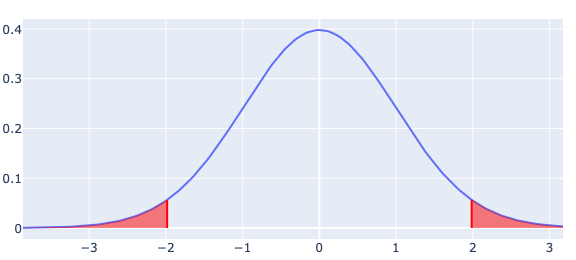
\includegraphics[width=0.8\textwidth]{rejectionRegion2}
	\caption{Rejection region (red) for the two-sided $t$ test with significance level $\alpha = 0.05$.}
\end{figure}

    
    \hypertarget{d-how-is-the-likelihood-ratio-test-related-to-the-one-sample-t-test-show-that-the-exact-rejection-region-of-the-likelihood-ratio-test-without-approximation-by-the-chi2-distribution-has-the-same-form-as-the-rejection-region-of-the-t-test.}{%
\subparagraph{\texorpdfstring{(d) How is the likelihood ratio test
related to the one-sample \(t\)-test? Show that the exact rejection
region of the likelihood ratio test (without approximation by the
\(\chi^2\)-distribution) has the same form as the rejection region of
the
\(t\)-test.\\[2ex]}{(d) How is the likelihood ratio test related to the one-sample t-test? Show that the exact rejection region of the likelihood ratio test (without approximation by the \textbackslash chi\^{}2-distribution) has the same form as the rejection region of the t-test.}}\label{d-how-is-the-likelihood-ratio-test-related-to-the-one-sample-t-test-show-that-the-exact-rejection-region-of-the-likelihood-ratio-test-without-approximation-by-the-chi2-distribution-has-the-same-form-as-the-rejection-region-of-the-t-test.}}

    Observe that given \(\Lambda(x_1, \ldots, x_n)\), we reject the null
hypothesis if, for some value \(k \in (0,1)\),
\[\Lambda(x_1, \ldots, x_n) = \left(\frac{\sum_i (x_i - \overline{x})^2}{\sum_i x_i^2} \right)^{n/2} < k\]
which occurs if and only if
\[ \frac{\sum_i x_i^2}{\sum_i (x_i - \overline{x})^2} = \frac{\hat{\sigma}^2 + \frac{n}{n-1}\overline{x}^2}{\hat{\sigma}^2} > k^{-2/n} =: k'\]
which can be rewritten as
\[ \frac{\overline{x}^2}{\hat{\sigma}^2/n} > (n-1)(k'-1) =: k'' \] and
since both sides are greater or equal than zero (because \(k' > 1\)),
this occurs if and only if
\[ \left|\frac{\overline{x}}{\sqrt{\hat{\sigma}^2/n}}\right| > \sqrt{k''}\]

which is the same rejection region as above. Hence, the exact
distribution of the likelihood ratio is the same as the \(t\) test and,
consequently, both test are equivalent.

    \hypertarget{e-analyze-either-by-simulation-or-by-computation-how-large-the-error-is-if-you-use-the-asymptotic-distribution-of-the-likelihood-ratio-statistic-versus-the-exact-distribution-as-in-d.}{%
\subparagraph{(e) Analyze either by simulation or by computation how
large the error is if you use the asymptotic distribution of the
likelihood ratio statistic versus the exact distribution as in
(d).\\[2ex]}\label{e-analyze-either-by-simulation-or-by-computation-how-large-the-error-is-if-you-use-the-asymptotic-distribution-of-the-likelihood-ratio-statistic-versus-the-exact-distribution-as-in-d.}}

    The error the asymptotic distribution is making is quite large, compared
to the aimed confidence level.

By simulating 5000 samples of size 100 from a standard normal
distribution, I tested the null hypothesis \(H_0: \mu = 0\) against
\(H_A: \mu \neq 0\) using the exact distribution and the approximate
one, for a significance level \(\alpha = 0.05\). For each of these
samples, the \(\Lambda\) and \(t\) statistics were computed and then
confronted to their respective rejection thresholds. After the
simulation, the exact distribution rejected \(H_0\) around 5\% of the
time, as expected from the confidence level. On the contrary, the
asymptotic distribution rejected 30\% of all the hypothesis tested.
Moreover, the error was increasing in the sample size, with 44\% of null
hypothesis rejected when sample size equals 1,000 and 48\% when the
sample size was 10,000.

Another aspect to consider is that these tests are highly susceptible to
the underlying standard deviation and the type-I error is increasing in
its value. The approximate distribution, moreover, is the most affected
by this behaviour. Increasing the standard deviation from 1 to 1.1 only
affects the type-I error of the exact test by 1 percentage point (from
5\% to 6\%). However, the asymptotic test increases is false rejection
rate up to 79\%. Increasing \(\sigma\) again in one tenth ends up with
an useless aymptotic test, with a false discovery rate of 100\%, against
a 7\% of the exact test.

    
\end{document}
